\documentclass[12pt]{article}
\usepackage[utf8]{inputenc}
\usepackage{parskip}

\usepackage[bottom]{footmisc}
\usepackage{titlesec}

\usepackage{graphicx}
\usepackage{subcaption}
\usepackage{wrapfig}

\usepackage{mathtools}
\def\is{\coloneqq}

\usepackage{algorithm,algorithmicx}
\usepackage[noend]{algpseudocode}

\begin{document}

\section{Segmentation is my fault}
\subsection{Introducción y presentación del trabajo realizado}

La segmentación de imágenes de forma es un problema abierto en el área de
\emph{visión artificial} que dada la variedad de sus aplicaciones posee varios
intereses en conflicto al querer desarrollar un algoritmo definitivo para ésta.
Un algoritmo eficiente que requiera tiempo y memoria lineal puede ser útil para
procesamiento de video en tiempo real sacrificando la calida del resultado,
mientras que otro enfoque más costoso puede ser útil a la hora de ofrecer una
herramienta que facilite labores artísticos (separación automática de los
objetos en una escena, por ejemplo).

\begin{figure}[h]
	\centering
	\begin{subfigure}{0.4\linewidth}
		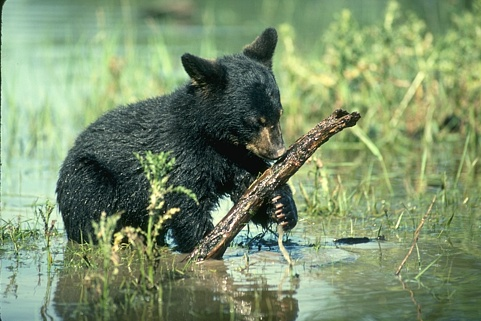
\includegraphics[width=\linewidth]{segmentation/entradas-posta/oso}
		\caption{Entrada}
	\end{subfigure}
	\begin{subfigure}{0.4\linewidth}
		\includegraphics[width=\linewidth]{segmentation/salidas/{0.8.oso.jpg.600.100}.png}
		\caption{Segmentación}
	\end{subfigure}
	\caption{$\sigma = 0.8,\ k = 600,\ g = 100$.}
\end{figure}

El algoritmo a implementar es el propuesto por \textbf{Pedro F.  Felzenszwalb}
y \textbf{Daniel P. Huttenlocher} en su trabajo \textsc{Efficient Graph-Based
Image Segmentation}. Éste algoritmo construye un grafo grilla con cada píxel en
su propio segmento y luego uno los segmentos golosamente dada una condición de
``similaridad suficente'' entre ellos. Para mejorar los resultados del
algoritmo se implementaron dos pasos de pre y post procesamiento.

El preprocesamiento consiste de un desenfoque gaussiano de dos pasadas. Éste se
implementó dentro del programa entregado luego de notar que desenfocar la
imagen y luego guardarla en el formato de entrada propuesto por la cátedra
resultaba en artefactos indeseables propios del bajo rango de valores de cada
pixel. El sigma de desenfoque puede ser modificando variando el segundo
parámetro pasado al ejecutable.

El postprocesamiento es una segunda pasada por las aristas del grafo forzando
la unión de todos los componentes suficientemente chicos. El significado de
``suficientemente chico'' se puede modificar variando el tercer parámetro
pasado al ejecutable. El parámetro es relativo a la resolución de la imagen a
procesar, un valor de $1$ eliminará todas las componentes que posean menos del
$100\%$ de los píxeles, uno de $10$ todas las que posean menos del $10\%$.
Llamaremos $g$ a este parámetro dado que cuanto mayor es su valor mayor es la
\emph{granularidad} de la segmentación resultante\footnote{Efectivamente el
parámetro pone un límite superior a la cantidad de segmentos que puede tener la
segmentación.}.

El algoritmo en sí posee un valor $k$ que representa la ``soltura'' a la hora
de comparar componentes para decidir si unirlas o no. Éste parámetro es el
primero que recibe el ejecutable entregado.

La elección de colores para las segmentaciones mostradas en este informe se
realizó aprovechándose de detalles implementativos. Esta elección nos permite
que los colores sean estables al variar tanto $k$ cómo $g$, lo cuál permitió
crear los videos adjuntos a este informe.

\subsection{Presentación informal e intuitiva del algoritmo}

El algoritmo implementado construye un \emph{grafo grilla} a partir de la
imagen proporcionada y luego recorre las aristas del mismo de menor a mayor
uniendo las compomentes de cada lado de la arista. La motivación es simple,
procesar los píxeles más similares al principio nos forzará a recorrer las
regiones de la imagen desde las de menos variabilidad hasta las que sean
básicamente ruido blanco.

Para tomar la decisión de si unir o no dos componentes se propone calcular la
\emph{diferencia interna} de una componente de la siguiente forma:

\[Int(C) = \max_{a \in AGM(C_V, C_E)} p(a)\]

Dónde $AGM(V, E)$ es el árbol generador mínimo del subgrafo de la componente
$C$, $C_V$ son los vértices de la componente V, $C_E$ son los ejes de la
componente $C$ y $p(e)$ es la función que determina el peso de una
arista\footnote{Dependiendo el espacio de color de la imagen y la forma en la
que se representen los mismos puede haber muchas funciones que tenga sentido
evaluar como $p$.}.

\begin{figure}[h]
	\centering
	\includegraphics[width=0.9\linewidth]{graficos/grilla}
	\caption{Grafo grilla con 8-vecindad.}
\end{figure}

Dado todo esto, dos componentes que limiten en un par de píxeles se unirán si
la diferencia en el límite está dentro de la tolerancia común de las mismas, es
decir si $\textit{diff} \geq Int(C_1) + \tau(C_1) \land \textit{diff} \geq
Int(C_2) + \tau(C_2)$, dónde $\tau(C)$ es la función que le da juego\footnote{\
En el sentido de que suma cierta holgura que permite unir componentes de que
otro parecerían demasiado distintas, cosa que es común con componentes
pequeñas} a la componente. La función propuesta para $\tau(C)$ es la siguiente:

\[\tau(C) = \frac{K}{|C_V|}\]

La que nos ofrece un valor cercano a $K$ para compontentes muy chicas y uno
cercano a $0$ para componentes muy grandes. Ésto fuerza a tener evidencias
claras de que dos componentes son en realidad la misma al ser estas muy grandes
pero nos permite un montón de juego en las primeras etapas.

\subsubsection{Entonces. ¿Cuál es el algoritmo aquí propuesto?}

Construiremos una primera aproximación burda (ubicando cada píxel en su propia
componente) y lo refinaremos preguntándonos si dado un par de componentes
unidas por un eje éstas no deberían en realidad unirse. A la hora de ejecutar
un algorimo así de goloso es importante el orden en el cuál se toman las
aristas a procesar. El obvio (y el utilizado por nosotros) es de menor a mayor
peso\footnote{En una implementación que requiera un tiempo de procesamiento
lineal se puede utilizar un \emph{Counting Sort} sabiendo cuál es la mayor
diferencia posible (256 en el caso de la entrada de la cátedra).}.

Entonces, sumando todos los procesos antes mencionados podemos construir una
suerte de vista aérea de nuestro algoritmo (que nos será útil para luego
ahondar en la implementación de cada parte).

\begin{enumerate}
	\item Cargar la entrada
	\item \textbf{Opcional:} Realizar un desenfoque para evitar
	      ciertos defectos.
	\item Construir el grafo grilla de la entrada, usando la diferencia
	      de intensidades entre píxeles vecinos como peso de cada arista.
	\item Ordenar las aristas construídas por peso.
	\item Construir la solución inicial, asignando a cada píxel (vértice
	      del grafo) en supropia componente.
	\item Por cada arista (de menor a mayor) determinar si los píxeles que
	      une deberían pertenecer a la misma componente. Si es así unirlos.
	\item \textbf{Opcional:} Por cada arista (de menor a mayor) si alguna
	      de las componentes que une es menor al $\frac{100}{g}\%$ de la
	      imagen entonces unir éstas.
	\item Imprimir la salida en el formato deseado, construir colores de
	      ser necesario, etc.
\end{enumerate}

\subsection{El algoritmo (y sus partes)}

En esta sección mostraremos el pseudocódigo correspondiente a este trabajo en
conjunto con información sobre detalles implementativos.

Los algoritmos acá mostrados usan todos alguna implementación de la estructura
\textsc{Disjoint-Set} que posee los siguientes observadores y operaciones:

\begin{itemize}
	\item \Call{Nuevo}{$s$}
		--- Retorna un nuevo \textsc{Disjoint-Set} con $s$ elementos.
	\item \Call{Buscar}{ds, $e$}
		--- Retorna el identificador de la componente de $e$.
	\item \Call{Unir}{ds, $a$, $b$}
		--- Une al componente que contiene a $a$ con el componente que
		contiene a $b$.
	\item \Call{Tamaño}{ds, $e$}
		--- Retorna el tamaño (en cantidad de elementos) de la
		componente que contiene a $e$.
\end{itemize}

\subsubsection{Desenfoque}

La implementación del desenfoque depende se realiza generando el \emph{kernel}
con el $\sigma$ apropiado. Y aprovecharnos de la \emph{separabilidad} del
filtro para hacer una convolución en cada eje en lugar de tener que usar la
matriz completa. Por otro lado elegimos limitar la cantidad de términos de la
máscara a los que naturales desde $0$ hasta $\lceil 4 \sigma \rceil$ cuando
necesitamos valores negativos de la normal los reflejamos en el \emph{kernel}
calculado. El tope que escojemos hace que los coeficientes fuera del
\emph{kernel} sean menores a $e^{-8}$ que son suficentemente pequeños cómo para
no resultarnos relevantes.

\begin{algorithm}[H]
\caption{Algoritmo para realizar un desenfoque gaussiano}
\begin{algorithmic}[1]
\Statex{}
\Function{Desenfocar}{$w$, $h$, imagen, $\sigma$}`
	\Statex{} \Comment{} Por simpleza no están los chequeos de límites en la imagen
	\State{} $\text{kernel} \is []$
	\For{$i \is 0$ to $\lceil 4 \sigma \rceil + 1$}
	\Comment{Coefficientes de la normal a usar}
		\State{} $\text{kernel}[i]
			\is \frac{1}{\sqrt{2\pi\sigma^2}}e^{-\frac{i^2}{2\sigma^2}}$
	\EndFor{}
	\For{$y \is 0$ to $h$}
		\Comment{} Convolución horizontal
		\For{$x \is 0$ to $w$}
			\State{} $\text{sum} \is 0$
			\For{$i \is 0$ to $|\text{kernel}|$}
				\State{} $\text{sum} \is \text{sum}
					+ \text{kernel}[i] \times (
						\text{imagen}[y][x - 1]
						+ \text{imagen}[y][x + 1]
					)$
			\EndFor{}
			\State{} $\text{imagen}[y][x] \is \text{sum}$
		\EndFor{}
	\EndFor{}
	\For{$y \is 0$ to $h$}
		\Comment{} Convolución vertical
		\For{$x \is 0$ to $w$}
			\State{} $\text{sum} \is 0$
			\For{$i \is 0$ to $|\text{kernel}|$}
				\State{} $\text{sum} \is \text{sum}
					+ \text{kernel}[i] \times (
						\text{imagen}[y - 1][x]
						+ \text{imagen}[y + 1][x]
					)$
			\EndFor{}
			\State{} $\text{imagen}[y][x] \is \text{sum}$
		\EndFor{}
	\EndFor{}
\EndFunction{}
\end{algorithmic}
\end{algorithm}

\subsubsection{Construcción del grafo}

Para construir el grafo utilizamos la 8-vecindad cómo ya dijimos anteriormente.
Una vez cargada la imagen podemos recorrer todos los píxeles (que serán
vértices de nuestro grafo) y agregar los ejes necesarios.

\begin{algorithm}[H]
\caption{Algoritmo para construir el grafo a segmentar}
\begin{algorithmic}[1]
\Statex{}
\Function{Construir-Grafo}{$w$, $h$, imagen}
	\Statex{} \Comment{} Describimos a los ejes como \{desde, hasta, peso\}
	\State{} $\text{ejes} \is \emptyset$
	\For{$y \is 0$ to $h$}
		\For{$x \is 0$ to $w$}
			\State{} $p_o \is \{x, y\}$
			\State{} $p_e \is \{x + 1, y\}$
			\If{$p_e$ está en los límites de la imagen}
				\State{} $\text{dif}
					\is \Call{Diferencia}{p_o,\ p_e,\ \text{imagen}}$
				\State{} \Call{Agregar}{ejes, \{$p_o$, $p_e$, dif\}}
			\EndIf{}
			\State{} $p_{sw} \is \{x - 1, y + 1\}$
			\If{$p_{sw}$ está en los límites de la imagen}
				\State{} $\text{dif}
					\is \Call{Diferencia}{p_o,\ p_{sw},\ \text{imagen}}$
				\State{} \Call{Agregar}{ejes, \{$p_o$, $p_{sw}$, dif\}}
			\EndIf{}
			\State{} $p_s \is \{x, y + 1\}$
			\If{$p_s$ está en los límites de la imagen}
				\State{} $\text{dif}
					\is \Call{Diferencia}{p_o,\ p_s,\ \text{imagen}}$
				\State{} \Call{Agregar}{ejes, \{$p_o$, $p_s$, dif\}}
			\EndIf{}
			\State{} $p_{se} \is \{x + 1, y + 1\}$
			\If{$p_{se}$ está en los límites de la imagen}
				\State{} $\text{dif}
					\is \Call{Diferencia}{p_o,\ p_{se},\ \text{imagen}}$
				\State{} \Call{Agregar}{ejes, \{$p_o$, $p_{se}$, dif\}}
			\EndIf{}
		\EndFor{}
	\EndFor{}
	\State{} \Return{} ejes
\EndFunction{}
\end{algorithmic}
\end{algorithm}

\subsubsection{Segmentación}

Con los ejes ya ordenados el proceso de segmentar la imagen es muy simple.
$\tau(C)$ es la función que dado un identificador de componente indica el
factor de juego que le corresponde a esa componente.

\begin{algorithm}[H]
\caption{Algoritmo segmentar el grafo generado}
\begin{algorithmic}[1]
\Statex{}
\Function{Segmentar}{$w$, $h$, ejes}
	\State{} $\text{ds} \is \Call{Nuevo}{w \times h}$
	\State{} $\text{umbral} \is [\tau(0), \tau(1), \dots, \tau(w \times h - 1)]$
	\For{$\text{eje} \in \text{grafo}$ (de menor a mayor peso)}
		\State{} $C_a \is \Call{Buscar}{\text{ds},\ \text{eje}.\text{desde}}$
		\State{} $C_b \is \Call{Buscar}{\text{ds}\, \text{eje}.\text{hasta}}$
		\If{$\text{eje}.\text{peso} \leq \text{umbral}[C_a]
			\land \text{eje}.\text{peso} \leq \text{umbral}[C_b]$}
			\State{} \Call{Unir}{ds, $C_a$, $C_b$}
			\State{} $C_a \is \Call{Buscar}{\text{ds},\ C_a}$
			\State{} $\text{umbral}[C_a] \is \Call{Tamaño}{\text{ds},\ C_a}
				+ \tau(C_a)$
		\EndIf{}
	\EndFor{}
	\State{} \Return{} ds
\EndFunction{}
\end{algorithmic}
\end{algorithm}

\subsubsection{Simplificación Greedy}

Una vez segmentada la imagen se puede realizar un paso final que elimine las
componentes más pequeñas. El recorrer las aristas de menor a mayor peso hace
que las componentes que se unifiquen siempre lo hagan por la arista más liviana
de su frontera (que es lógico suponer pertenece a la componente limítrofe más
parecida).

\begin{algorithm}[H]
\caption{Algoritmo para eliminar segmentos pequeños}
\begin{algorithmic}[1]
\Statex{}
\Function{Simplificar}{$w$, $h$, ds, ejes, $g$}
	\State{} $\text{min} \is \frac{g}{w \times h}$
	\For{$\text{eje} \in \text{ejes}$ (de menor a mayor peso)}
		\If{$\Call{Tamaño}{\text{ds, eje}_a} < \text{min}
		     \vee \Call{Tamaño}{\text{ds, eje}_b} < \text{min}$}
			\State{} $C_a \is \Call{Buscar}{\text{ds, eje}_a}$
			\State{} $C_b \is \Call{Buscar}{\text{ds, eje}_b}$
			\If{$C_a \neq C_b$}
				\State{} \Call{Unir}{ds, $C_a$, $C_b$}
			\EndIf{}
		\EndIf{}
	\EndFor{}
\EndFunction{}
\end{algorithmic}
\end{algorithm}

\subsubsection{Vista aérea del algoritmo}

A modo de unificar todos los pasos ya expuestos en detalle podemos resumir la
operación del algoritmo en pocas líneas:

\begin{algorithm}[H]
\caption{Algoritmo para segmentar con todos los pasos comentados}
\begin{algorithmic}[1]
\Statex{}
\Function{Simplificar}{$w$, $h$, imagen, $\sigma$, $k$, $g$}
	\State{} \Call{Desenfocar}{$w$, $h$, imagen, $\sigma$}
	\State{} $\text{ejes} \is \Call{Construir-Grafo}{w,\ h,\ \text{imagen}}$
	\State{} \Call{Ordenar}{ejes}
	\State{} $\text{segmentación} \is \Call{Segmentar}{w,\ w,\ \text{ejes}}$
	\State{} \Call{Simplificar}{$w$, $h$, segmentación, ejes, $g$}
	\State{} \Return{} segmentacion
\EndFunction{}
\end{algorithmic}
\end{algorithm}

\subsection{Estructuras para implementar \textsc{Disjoint-Set}}

Como parte del trabajo la cátedra requirió implementar el \textsc{Disjoint-Set}
con 3 estructuras distintas, las listamos en conjunto con la complejidad de las
operaciones antes descriptas:

\begin{itemize}
	\item Representado como arreglo de componentes
	\begin{itemize}
		\item \Call{Nuevo}{s}: $O(s)$
		\item \Call{Buscar}{ds, $e$}: $O(1)$
		\item \Call{Unir}{ds, $a$, $b$}: $O(n)$
		\item \Call{Tamaño}{ds, $e$}: $O(1)$
	\end{itemize}
	\item Representado como árbol
	\begin{itemize}
		\item \Call{Nuevo}{s}: $O(s)$
		\item \Call{Buscar}{ds, $e$}: $O(n)$
		\item \Call{Unir}{ds, $a$, $b$}: $O(1)$
		\item \Call{Tamaño}{ds, $e$}: $O(1)$
	\end{itemize}
	\item Representado como árbol con \emph{path compression}
	\begin{itemize}
		\item \Call{Nuevo}{s}: $O(s)$
		\item \Call{Buscar}{ds, $e$}: $O(\alpha(s))$
			\textbf{(amortizado)}
		\item \Call{Unir}{ds, $a$, $b$}: $O(\alpha(s))$
			\textbf{(amortizado)}
		\item \Call{Tamaño}{ds, $e$}: $O(\alpha(s))$
			\textbf{(amortizado)}
	\end{itemize}
\end{itemize}

Sumado a esto, las representaciones de árbol pueden elegir si unir por mayor
rango o por mayor tamaño (en nuestro caso particular implementamos por mayor
tamaño).

\subsubsection{Resultados con distintos tamaños de imagen}

En este apartado buscamos determinar el comportamiento de nuestras
implementaciones dados diferentes tamaños de imagen. Queremos verificar en cada
uno de ellos como varía el timpo de ejecución. 

Usaremos 3 imagenes con dimensiones cuadradas por su facilidad para
redimensionarlas. Las resoluciones a utilizar serán $[100 \times
100\text{px},200 \times 200\text{px}, \dots, 700 \times 700\text{px}]$.

\begin{figure}[H]
	\centering
	\begin{subfigure}{0.3\linewidth}
		
\includegraphics[width=\linewidth]{segmentation/entradas-posta/mondrian}
		\caption{\texttt{mondrian.jpg}}
	\end{subfigure}
	\begin{subfigure}{0.3\linewidth}
		
\includegraphics[width=\linewidth]{segmentation/entradas-posta/edificios}
		\caption{\texttt{edificios.png}}
	\end{subfigure}
	\begin{subfigure}{0.3\linewidth}
		
\includegraphics[width=\linewidth]{segmentation/entradas-posta/bosque}
		\caption{\texttt{bosque.jpg}}
	\end{subfigure}
\end{figure}

Las 3 imágenes han sido seleccionadas para probar tres casos claros: (a)
posee varias regiones planas sobre las cuales el algoritmos ejecutará
\textsc{Union} muchas veces, (b) tiene una textura dominante que al no ser
del todo plana generará varios segmentos de pocos píxeles y (c) tiene muchos
pequeños detalles que harán que se generen montones de segmentos.

Los parámetros para cada corrida serán $k = 300$, $\sigma = 0.8$ sin paso de
simplificación. Para ver el efecto que tiene variar los parámetros en el tiempo
de ejecución tendremos una sección más adelante.

\begin{figure}[H]
	\centering
	\includegraphics[width=0.75\linewidth]{segmentation/experimentacion/distintas-fotos-arreglo}
	\caption{Segmentación implementando \textsc{Disjoint-Set} con arreglo.}
\end{figure}

\begin{figure}[H]
	\centering
	\includegraphics[width=0.75\linewidth]{segmentation/experimentacion/distintas-fotos-arbol}
	\caption{Segmentación implementando \textsc{Disjoint-Set} con un árbol.}
\end{figure}

\begin{figure}[H]
	\centering
	\includegraphics[width=0.75\linewidth]{segmentation/experimentacion/distintas-fotos-arbol-compr}
	\caption{Segmentación implementando \textsc{Disjoint-Set} con un árbol con compresión.}
\end{figure}

En los 3 algoritmos podemos observar un comportamiento similar, siendo el
algoritmo de árbol de compresión el que muestra un rendimiento superior
(alrededor de dos veces más rápido que el resto). Esto no se condice con la
complejidad teórica, pero puede deberse a que el eje X de los gráficos no
representa un cambio lineal en el tamaño de la entrada.

Otra cosa notable es que pese a las claras diferencias entre las imágenes todos
los algoritmos tienen un comportamiento similar dada una misma resolución de
imagen.

\subsubsection{Influencia de los parámetros}

Esta sección del informe analiza el rendimiento de las distintas
representaciones variando los parámetros $k$ y $g$\footnote{Valores de $\sigma$
mayores aumentarían el tiempo requerido de procesamiento pero ese procesamiento
se realiza antes de cualquier llamada a las estructuras que son relevantes a
esta sección del informe.}.

Dado que \textsc{Buscar} es considerablemente más simple en las
implementaciones con arreglo de componententes creemos que es esperable que
presente un rendimiento levemente superior para valores de $k$ y $g$ muy bajos
(dónde se realizan muy pocas llamadas a \textsc{Unir}).

Para realizar estos experimentos tomamos una sola imagen como entrada
(\texttt{autitos.jpg}) sobre la cuál experimentamos. La decisión de tomar una
única imagen fué debido a que queremos medir el efecto de los parámetros en una
imagen dónde estos tengan relevancia (en una imagen completamente plana variar
$k$ o $g$ no cambiaría la segmentación resultante, las llamadas a \textsc{Unir}
y \textsc{Buscar} serían siempre las mismas).

\begin{figure}[h]
	\centering
	\begin{subfigure}{0.4\linewidth}
		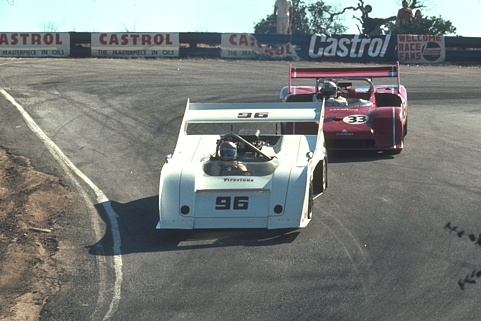
\includegraphics[width=\linewidth]{segmentation/entradas-posta/autitos}
		\caption{Entrada}
	\end{subfigure}
	\begin{subfigure}{0.4\linewidth}
		\includegraphics[width=\linewidth]{segmentation/salidas/{0.8.autitos.jpg.300.1000}.png}
		\caption{Segmentación}
	\end{subfigure}
	\caption{$\sigma = 0.8,\ k = 300,\ g = 1000$.}
\end{figure}

\subsubsection{Resultados variando $k$}

En el primer experimento decidimos medir el tiempo que tardaba el paso de
segmentación variando el $k$ de $0$ a $1200$ con incrementos de a $50$.

\begin{figure}[h]
	\centering
	\includegraphics[width=0.75\linewidth]{segmentation/experimentacion/variar-k}
	\caption{Tiempo incurrido por el proceso de segmentar al variar el $k$}
\end{figure}

Cuándo $k$ es $0$ el gráfico muestra que la segmentación realiza poco trabajo,
pero a partir de $50$ no muestra ninguna tendencia clara. Cómo la
experimentación se realizó con la misma entrada siempre esto da indicios de que
el coste de este trabajo no se ve influído más que por las características del
grafo grilla que se construye.

\subsubsection{Resultados variando $g$}

Dado que la granularidad varía su trabajo de acuerdo al $k$ elegido decidimos
tomar $k$ entre $0$ y $1200$ y variar el $g$ entre $1$ y $991$ en incrementos
de $10$.

\begin{figure}[h]
	\centering
	\includegraphics[width=0.75\linewidth]{segmentation/experimentacion/variar-g-arreglo}
	\caption{Tiempo incurrido por el proceso de simplificar al variar el $g$}
\end{figure}

Para $k=0$ vemos que cómo que el set resultante de la segmentación tenga
muchísimos conjuntos pequeños logra que el tiempo que requiera la
simplificación sea considerablemente mayor. También vemos que cada
implementación llega a un mínimo dado un $g$ suficientemente alto dónde el
costo de hacer las llamadas a \textsc{Tamaño} superan a las pocas llamadas a
\textsc{Unir} resultantes de los chequeos.

\begin{figure}[h]
	\centering
	\includegraphics[width=0.75\linewidth]{segmentation/experimentacion/variar-g-arbol}
	\caption{Tiempo incurrido por el proceso de simplificar al variar el $g$}
\end{figure}

Tomar el árbol como representación el caso de $k=0$ arroja resultados
interesantes. Dado que no se comprime el árbol cuanto menos se unifiquen las
componentes menor es el coste de \textsc{Tamaño} que internamente realiza una
llamada a \textsc{Buscar}. Lamentablemente cómo no experimentamos con mayor
finura en los valores de $k$ entre $1$ y $150$ no podemos decir nada sobre cuál
sea la tendencia que toma el gráfico en ese rango, sí vemos una tendencia más
clara para el resto de los valores que tenemos información.

\clearpage

\begin{figure}[h]
	\centering
	\includegraphics[width=0.75\linewidth]{segmentation/experimentacion/variar-g-arbol-compr}
	\caption{Tiempo incurrido por el proceso de simplificar al variar el $g$}
\end{figure}

Finalmente, en la simplificación usando la representación de árbol con
compresión volvemos a ver las tendencias de la representación de arreglo pero
con tiempos la mitad de grandes. Dado que los costes teóricos deberían ser
diferentes pero vemos tendencias muy similares esto nos da indicios de que
nuestro experimento no supo elegir valores que evidencien esas
diferencias\footnote{O que nuestras implementaciones tienen errores que hacen
que no funcionen de la forma esperada.}

\clearpage

\subsection{Análisis de resultados}

Sumado a la comparación entre distintas implementaciones del
\textsc{Disjoint-Set} en esta sección mostraremos segmentaciones resultantes de
ejecutar el algoritmo con distintos parámetros. También se ofrecen adjuntos
tres videos dónde se varía cada uno de los parámetros mientras se fijan los
otros dos\footnote{Dado que la forma en la que elegimos los colores no resultó
estable respecto de variar $\sigma$ el video dónde se lo varía podría resultar
molesto para personas con fotosensibildad.}.

\begin{figure}[h]
	\centering
	\begin{subfigure}{0.4\linewidth}
		
\includegraphics[width=\linewidth]{segmentation/entradas-posta/sintetico}
		\caption{Entrada}
	\end{subfigure}
	\begin{subfigure}{0.4\linewidth}
		\includegraphics[width=\linewidth]{segmentation/salidas/{0.8.sintetico.png.500.1000}.png}
		\caption{Segmentación}
	\end{subfigure}
	\caption{$\sigma = 0.8,\ k = 500,\ g = 1000$.}
\end{figure}

Una buena segmentación es un concepto difícil de definir, dado que depende el
nivel de granularidad deseado ciertos segmentos pueden resultar útiles o no
(ventanas en edificios, ojos en personas, letras individuales en una hoja,
etc). Cómo nuestro algoritmo sólo percibe la intensidad de cada píxel se pierde
información propia del color en la transformación que nos genera casos de error
que podrían salvarse de otro modo.

\subsubsection{Errores esperables}

Escojer un bien el valor de $\sigma$ resulta importante para eliminar ciertas
imperfecciones. Valores de entre $0.4$ t $0.8$ fueron los que utilizamos para
ver los resultados\footnote{Se puede correr \texttt{make ver\_todos} en
\texttt{segmentation} para ver los resultados con $\sigma = 0.8$, $k = 600$ y
sin pasada de simplificación. También se pueden pasar los valores como
parámetro en la forma \texttt{make BLUR=$\sigma$ K=$k$ MIN=$g$ ver\_todos}.}.

En las siguientes imágenes se pueden apreciar distintas segmentaciones de uno
de las imágenes que no pudimos encontrar un conjunto de parámetros que ofrezcan
una segmentación razonable. Dado que la evidente diferencia de color no se
traslada a la entrada en escala de grises. Puede observarse cómo el proceso de
simplificación mantiene algunos de los limites de la imagen original para
valores de $k$ muy bajos y cómo pu puede ser útil eliminar segmentos demasiado
chicos con esa técnica en lugar de elevar el $k$ perdiendo los segmentos del
insecto.

\begin{figure}[h]
	\centering
	\begin{subfigure}{0.4\linewidth}
		
\includegraphics[width=\linewidth]{segmentation/entradas-posta/mariquita}
		\caption{Entrada}
	\end{subfigure}
	\begin{subfigure}{0.4\linewidth}
		
\includegraphics[width=\linewidth]{segmentation/informe/mariquita}
		\caption{Entrada en escala de grises}
	\end{subfigure}
	\begin{subfigure}{0.4\linewidth}
		\includegraphics[width=\linewidth]{segmentation/salidas/{0.0.mariquita.jpg.6000.-1}.png}
		\caption{$\sigma = 0,\ k = 6000$}
	\end{subfigure}
	\begin{subfigure}{0.4\linewidth}
		\includegraphics[width=\linewidth]{segmentation/salidas/{0.0.mariquita.jpg.0.1000}.png}
		\caption{$\sigma = 0,\ k = 0,\ g = 1000$}
	\end{subfigure}
	\begin{subfigure}{0.4\linewidth}
		\includegraphics[width=\linewidth]{segmentation/salidas/{0.0.mariquita.jpg.600.-1}.png}
		\caption{$\sigma = 0,\ k = 600$}
	\end{subfigure}
	\begin{subfigure}{0.4\linewidth}
		\includegraphics[width=\linewidth]{segmentation/salidas/{0.0.mariquita.jpg.600.1000}.png}
		\caption{$\sigma = 0,\ k = 600,\ g = 1000$}
	\end{subfigure}
	\caption{Distintas configuraciones con distintos tipos de error,
	aquellas que no especifican valores para $g$ no tuvieron paso de
	simplificación.}
\end{figure}

\clearpage

La importancia del desenfoque no es evidente en todas las imágenes, la
siguiente escena muestra un defecto que ocurre cuando las fotos tienen mucho
grano:

\begin{figure}[h]
	\centering
	\begin{subfigure}{0.3\linewidth}
		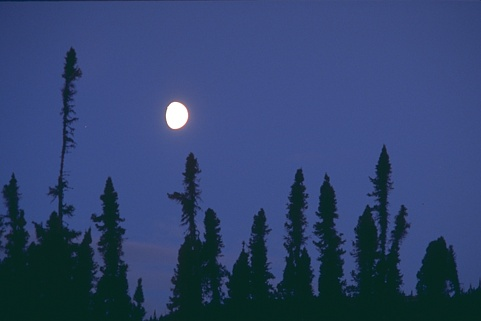
\includegraphics[width=\linewidth]{segmentation/entradas-posta/noche}
		\caption{Entrada}
	\end{subfigure}
	\begin{subfigure}{0.3\linewidth}
		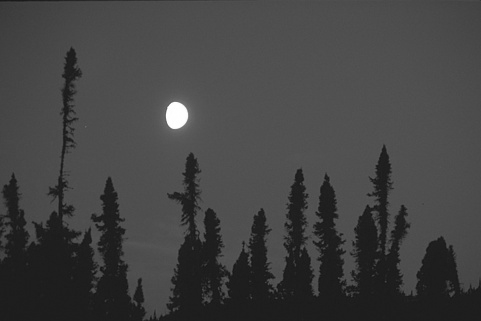
\includegraphics[width=\linewidth]{segmentation/informe/noche}
		\caption{Escala de grises}
	\end{subfigure}
	\begin{subfigure}{0.3\linewidth}
		\includegraphics[width=\linewidth]{segmentation/salidas/{0.0.noche.jpg.600.-1}.png}
		\caption{$\sigma = 0,\ k = 600$}
	\end{subfigure}
	\begin{subfigure}{0.3\linewidth}
		\includegraphics[width=\linewidth]{segmentation/salidas/{0.2.noche.jpg.600.-1}.png}
		\caption{$\sigma = 0.2,\ k = 0$}
	\end{subfigure}
	\begin{subfigure}{0.3\linewidth}
		\includegraphics[width=\linewidth]{segmentation/salidas/{0.4.noche.jpg.600.-1}.png}
		\caption{$\sigma = 0.4,\ k = 600$}
	\end{subfigure}
	\begin{subfigure}{0.3\linewidth}
		\includegraphics[width=\linewidth]{segmentation/salidas/{0.6.noche.jpg.600.-1}.png}
		\caption{$\sigma = 0.6,\ k = 600$}
	\end{subfigure}
	\begin{subfigure}{0.4\linewidth}
		\includegraphics[width=\linewidth]{segmentation/salidas/{0.8.noche.jpg.600.-1}.png}
		\caption{$\sigma = 0.8,\ k = 600$}
	\end{subfigure}
	\begin{subfigure}{0.4\linewidth}
		\includegraphics[width=\linewidth]{segmentation/salidas/{1.0.noche.jpg.600.-1}.png}
		\caption{$\sigma = 1,\ k = 600$}
	\end{subfigure}
	\caption{Segmentación de una escena simple con grano.}
\end{figure}

\clearpage

\subsubsection{Resultados favorables}

\begin{figure}[h]
	\centering
	\begin{subfigure}{0.3\linewidth}
		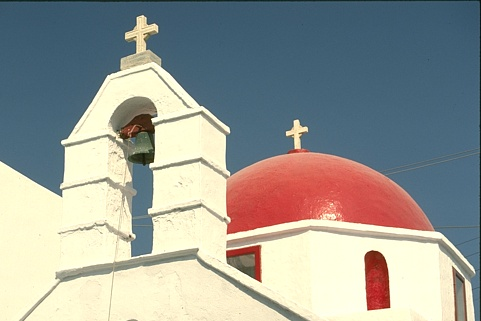
\includegraphics[width=\linewidth]{segmentation/entradas-posta/iglesia}
		\caption{Entrada}
	\end{subfigure}
	\begin{subfigure}{0.3\linewidth}
		\includegraphics[width=\linewidth]{segmentation/salidas/{0.8.iglesia.jpg.600.-1}.png}
		\caption{$\sigma = 0.8,\ k = 600$}
	\end{subfigure}
	\begin{subfigure}{0.3\linewidth}
		\includegraphics[width=\linewidth]{segmentation/salidas/{0.8.iglesia.jpg.600.1000}.png}
		\caption{$g = 1000$}
	\end{subfigure}
	\caption{Segmentacion de \texttt{iglesia.jpg}}
\end{figure}

\begin{figure}[h]
	\centering
	\begin{subfigure}{0.3\linewidth}
		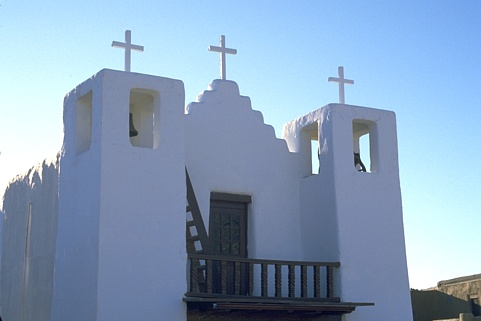
\includegraphics[width=\linewidth]{segmentation/entradas-posta/iglesia_2}
		\caption{Entrada}
	\end{subfigure}
	\begin{subfigure}{0.3\linewidth}
		\includegraphics[width=\linewidth]{segmentation/salidas/{0.8.iglesia_2.jpg.600.-1}.png}
		\caption{$\sigma = 0.8,\ k = 600$}
	\end{subfigure}
	\begin{subfigure}{0.3\linewidth}
		\includegraphics[width=\linewidth]{segmentation/salidas/{0.8.iglesia_2.jpg.600.1000}.png}
		\caption{$g = 1000$}
	\end{subfigure}
	\caption{Segmentacion de \texttt{iglesia\_2.jpg}}
\end{figure}

\begin{figure}[h]
	\centering
	\begin{subfigure}{0.3\linewidth}
		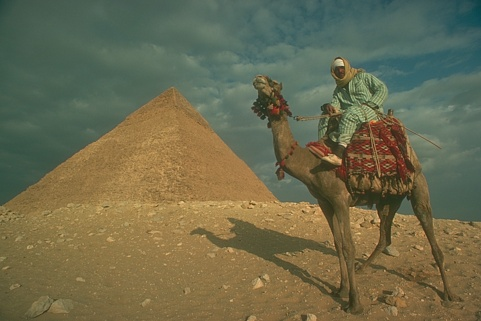
\includegraphics[width=\linewidth]{segmentation/entradas-posta/piramide_camello}
		\caption{Entrada}
	\end{subfigure}
	\begin{subfigure}{0.3\linewidth}
		\includegraphics[width=\linewidth]{segmentation/salidas/{0.8.piramide_camello.jpg.300.-1}.png}
		\caption{$\sigma = 0.8,\ k = 300$}
	\end{subfigure}
	\begin{subfigure}{0.3\linewidth}
		\includegraphics[width=\linewidth]{segmentation/salidas/{0.8.piramide_camello.jpg.300.1000}.png}
		\caption{$g = 1000$}
	\end{subfigure}
	\caption{Segmentacion de \texttt{piramide\_camello.jpg}}
\end{figure}

Cómo puede observarse, dado suficiente contraste el algoritmo genera
segmentaciones razonables, aunque por usar la 8-vecindad de cada píxel
construye pequeños segmentos en lugares quese ven cortados por una sombra.

\subsection{Conclusiones y trabajo futuro}

Con lo expuesto anteriormente está claro que el resultado de esta técnica es
muy sensible a los parámetros dados y a la claridad de la imagen de entrada.
Buscar heurísticas para encontrar éstos es un camino posible para facilitar el
uso del algoritmo así cómo otras formulaciones para la diferencia entre píxeles
y para $\tau(C)$.

Otro punto en el cual creemos que faltó trabajo es en utilizar diferentes
imágenes para ver cómo afectan al tiempo dadas las distintas implementaciones.
de \textsc{Disjoint-Set}. Creemos también que los videos que complementan éste
informe resultan útiles para entender las cualidades de la técnica. Pero dado
que la selección de colores no es estable respecto de $\tau$ una estrategia
mejor para construir las visualizaciones variando los parámetros es algo que
creemos nos faltó.


\section{Llenalo con super}

\subsection{Presentación informal del problema}
Dado un vendedor que cuenta con vehiculo propio que necesita moverse entre ciudades personalmente para vender sus productos, quiere buscar la manera más económica de realizar la tarea.

Si la distancias entre ciudades estan representadas en kilometros y el precio de la nafta es por litro queremos minimizar el costo en nafta de llegar de cada ciudad a las demas teniendo en cuenta las siguientes propiedades: 

\begin{enumerate}
	\item Las rutas que comunican las ciudades son bidireccionales.
	\item El precio de la nafta varia de ciudad en ciudad.
	\item El auto posee un limite de litros de nafta que puede cargar (60 litros).
	\item Se estima que cada litro de nafta alcanza para exactamente un kilometro de distancia.
	\item El auto siempre empieza descargado (Con 0 litros de combustible).
\end{enumerate}

El problema formalmente será representado como un grafo donde cada ciudad $c_i$ es un vertice con su respectivo precio por litro $p_i$ y donde cada distancia $d_{x,y}$ que comunica un par de ciudades ($c_x, c_y$) son las $m$ aristas del grafo.

Representado el $r_k$ como un camino posible entre dos ciudades en función del costo efectivo comprendido como la cantidad de litros $l_i$ que cargue de nafta por su respectivo precio $p_i$ queremos los caminos que cumplen que:

$\forall(c_x, c_y \in Ciudades)(r_{m}, r_k \in Caminos(c_x,c_y))\rightarrow(r_{m} < r_k)$

Es decir nos interesan todos los caminos minimos.

Una motivación razonable para resolver el problema sería entonces simplemente aplicar algoritmos conocidos de camino minimo, sin embargo esto no es posible con el grafo original.

Para empezar el precio al estar en función de los vertices, los costes no dependen solo de las distancias, sino de una multiplicación entre litros cargados por el precio.

Las rutas son bidireccionales, sin embargo dadas 2 ciudades $C_a$ y $C_b$ no se cumple que los costes $C_a \rightarrow C_b$ y $C_b \rightarrow C_a$ sean iguales.

Eso significa que necesitariamos una representación direccional si quisieramos hablar de costes efectivos. $Fig1, Fig2$ ilustran esta diferencia para 2 ciudades.

\begin{minipage}{0.5\textwidth}
	\includegraphics[width=\linewidth]{{graficos/bidireccional}.pdf}
	\captionof{figure}{bidireccional}
\end{minipage}
\begin{minipage}{0.5\textwidth}
	\includegraphics[width=\linewidth]{{graficos/direccional}.pdf}
	\captionof{figure}{direccional}
\end{minipage}

En particular $\forall(p_a \neq p_b) \rightarrow (p_a * d_{a,b} \neq p_b * d_{a,b}) $

Además los caminos minimos no necesariamente son simples, por ejemplo dadas 3 ciudades $C_a$, $C_b$ y $C_c$ y 2 rutas con distancia $d_{a,b}$ y $d_{a,c}$.

\begin{minipage}{0.5\textwidth}
	Tengo que si $p_a > p_b$ podría tener que evaluar si moverme allí para cargar nafta y volver es menos costoso, que ir directamente.
	
	En fig3 se ilustra un grafo donde el costo de ir de $C_A$ a $C_C$ directamente es $p_a * d_{a,c} = 750$.
	
	Mientras que el camino pasando por $C_b$ es:
	
	$C_a$ a $C_b$ a $C_a$ a $C_C$ = 450.
	
	Sin embargo esto motiva a analizar si existen transformaciones del grafo en la que aplicar algoritmos de camino minimo es posible.
\end{minipage}
\begin{minipage}{0.5\textwidth}
	\includegraphics[width=\linewidth]{{graficos/caminoNoSimple}.pdf}
	\captionof{figure}{CaminoNoSimple}
\end{minipage}


\subsubsection{Pautas de diseño}

El objetivo de este trabajo es plantear transformaciones de grafos que nos permitan aplicar algoritmos de camino minimo. Buscaremos establecer una cota de las dimensiones de nuestro nuevo grafo en función de la densidad y tamaño del grafo original.

Someteremos nuestro grafo a diferentes experimentos buscando comparar entre diferentes algoritmos de camino minimo cual de ellos se ajusta mejor. No explicaremos algoritmos de camino minimo como Dijkstra, Bellman-ford o Floyd-Warshall, se entienden por conocidos.

Finalmente Dijkstra, bellman-ford son algoritmos $1$ a $N$ (nodos), cuando nos refiramos a ellos como algoritmos $N$ a $N$, nos referimos justamente a ejecutarlos $N$ veces (Abordaremos este tema en detalle en secciones posteriores).

\subsubsection{En búsqueda de un algoritmo}

Buscamos dado un grafo $V$, obtener todos sus costos efectivos minimos $R$ para cada $(C_i, C_j)$ y ádemas queremos realizar dicha tarea empleando algoritmos de camino minimo, para esto se plantearán 2 funciones. La primera una funciòn $f(V) = V'$ que convierta nuestro grafo en función del costo efectivo a un nuevo grafo en el cual si se puedan aplicar algoritmos de camino minimo. Luego buscamos una función $g(R') = R$ que sepa interpretar los resultados del nuevo grafo como solución del original y obtener los resultados de $V$ que nos interesan.

Dadas ambas funciones el algoritmo que aplicaremos sobre V para obtener los resultados R consta de los siguientes pasos:

\begin{enumerate}
	\item $V' \is f(V)$
	\item $R' \is$ Aplicar un algoritmo de camino minimo a $V'$
	\item $R \is g(R')$
\end{enumerate}

Hablaremos en detalle de los pasos (1) y (3), mientras que en el paso (2) solo haremos aclaraciones.

\subsubsection{Transformación del grafo $f(V)$}

Para lograr esta tarea, necesitamos eliminar la noción del precio ya que los algoritmos de camino minimo solo saben operar en funciòn del peso de las aristas. Además paso las aristas resultantes que debemos obtener serìa conveniente que esten en función del costo efectivo.

Sabemos además que la cantidad de litros de nafta que puede llevar nuestro vehiculo esta acotada por una constante llamemos $W$ de 60 litros. 

Debido a que W es acotado una estrategia razonable sería lograr que $f(V)$ dependa de esta constante, ya que la complejidad de un algoritmo de camino minimo $N$ a $N$ es $O(n^3)$, si incluimos el costo de la transformación sería $O(W * n^3)$ y si $W$ es constante no influiría en nuestra complejidad.

Empezemos por redefinir los vertices, en $V'$ no puedo tener estados, no puedo estar en una ciudad $C_i$ con $X$ de nafta, y un precio $p_i$ para agregar litros.

Lo primero que haremos será multiplicar cara vertice $C_i$ por W estados posibles\footnote{Si $(W = 60)$ los estados son $61$, puedo estar en $C_i$ con: (0..60) lirtros de nafta.} entonces si:

$V$ posee  N nodos. 

$V'$ posee N * 61 tal que si $C_i$ es nodo en V $\rightarrow$ $\exists$ $\sum_{k=0}^{W} C'_{i * k}$ nodos en $V'$

por notación llamaremos $C'_{i_0}$ a $C'_{i_{60}}$ a nuestros vertices en $V'$ ahora bien necesitamos redefinir nuestras aristas en función del costo efectivo. Tendremos 2 tipos de aristas.

\begin{itemize}
	\item (1) que representa una arista de carga de combustible y comunica los $W$ estados de un nodo. Es razonable considerar que si yo estoy en una ciudad con k litros y quiero agregar un litro de nafta el costo será el precio de cargar nafta en dicha ciudad. Es trivial asumir que en general tendremos que dado un estado $C'_{i_k}$ el costo para ir a $C'_{i_{k+1}}$ será exactamente $p_i$ para toda $d_{k,k+1}$.
\end{itemize}

Es decir de nuestra transformaciòn tiene  $N * (W - 1$) aristas para movernos entre los estados $C'_{i_k}$

\begin{itemize}
	\item (2) que representa una arista de movimiento entre nodos $(C_A, C_B)$, en general por cada $d_{C_A,C_B} \in m$ de $V$ diremos que en $V'$ esto solo sucederá si se cumple que $C'_{A_k}$ $\exists$ $d'_{A_k,B_j}$ $\leftrightarrow$  $k - d_{A,B} = j$. Es decir ir de $C_A$ a $C_B$ solo es posible si la cantidad de litros con la que voy a llegar a B es la cantidad de litros que tenía en A menos la distancia. Y el costo de esta arista en particular es $0$ debido a que para que sea posible ya cargue combustible en A, lo que significa que ya pague el precio.
\end{itemize}

Con estas condiciones generamos $V'$, pero necesitamos comprobar si esta transformación es válida. Para ello nos alcanza con demostrar que los resultados $R$ de $V$ existen en $V'$ en particular nos alcanza con decir que $(R \subset R')$. Si esto sucede entonces $\exists$ $g(R')$ que transforma a $R$. No necesariamente trivial.

Imaginemos que existe costo efectivo minimo en $V$  $\exists costo_{min} \in (C_A,C_B)$ tal que no existe en $V'$.

De ser así existe una combinación de formas de cargar combustible en distintas $C_i$ tal que $\sum (p_i * l_i)$ no existe en $R'$ entonces existe alguna (o varias) formas de cargar combustible en una ciudad $(p_i * l_k)$ que no esta en $V'$

Sin embargo en $V'$ los W estados que representan un nodo son todas las formas de estar en una ciudad con $l_x$ litros previamente cargados.

Y agregar nuevos litros significa moverme entre los estados agregando para cada $C'_{i_k}$ el costo $p_i$ para ir al $C'_{i_{k+1}}$ es decir que agregar $l_k$ litros es $\sum_0^Y d'_{k,k+1}$ dado que $p_i$ = $d'_{k,k+1}$ es explicitamente $(l_k * p_i)$ para cualquier $l_k$ que mantenga el rango $W \in (0..61)$

Dado que $\forall (C'_{A_i}, C'_{B_j}) \exists d_{A_i,B_j}$ si se cumple el item \textbf{(2)} estoy representando todas las formas posibles de llegar a destino con $x$ combustible cargado mi estado inicial $C_A$ es $C'_{A_0}$\footnote{Es condición del problema que arranco con el tanque vacio.} y tengo todas las formas posibles de llegar a $C_{B}$ con (0..W) litros en el tanque, no perdi soluciones.

Sin embargo tengo soluciones de más, en particular tengo W formas distintas de llegar a $C_B$, y solo me interesa una. Abordaremos este tema en detalle cuando definamos $g(R')$. El algoritmo sería el siguiente:



\begin{algorithm}[H]
	\caption{$f(V)$}
	\begin{algorithmic}[1]
		\item[\textbf{Inicialización:}]
		\item[] \begin{itemize}
			\item[] $V_n = $ cantidad de nodos en V.
			\item[] $V_{aristas(i)} = $ tripla $(origen, destino, peso)$ de la i-esima arista.
			\item[] $W = 61$
		\end{itemize}
		\item[\textbf{Funciones auxiliares:}]
		\item[] \begin{itemize}
			\item[] \Call{AgregarArista}{$C_a,C_b,peso$} agrega $d_{C_a,C_b}$ al grafo $V'$
		\end{itemize}
		\Statex
		\Function{TransformarGrafo}{$V, n, m$}
		\State $V'_n \is V_n * W$
		\For{$(i \in (0..n))$}
		\Comment Aristas de carga de combustible
		\For{$(k \in (1..W))$}
		\State $C_{i_k} \is i * W + k$
		\State \Call{AgregarArista}{$C_{i_k} - 1,C_{i_k},peso$}
		\EndFor
		\EndFor
		\State
		
		\For{$(i \in (0..m))$}
		\State $C_a,C_b,d_{a,b} \is V_{aristas(i)}$
		\Comment Aristas de transición de nodos
		\For{$(k \in (1..W))$}
		\If{$k \geq d_{a,b}$}
		\Comment Agrego las aristas bidireccionalmente
		\State \Call{AgregarArista}{$C_a + k,C_b + k - d{a,b},0$}
		\State \Call{AgregarArista}{$C_b + k,C_a + k - d{a,b},0$}
		\EndIf
		\EndFor
		\EndFor
		
		\State \Return $V'$
		\EndFunction
	\end{algorithmic}
	\begin{description}
		\item[\textbf{Complejidad algorítmica:}] $O(W \times (n + m))$
	\end{description}
\end{algorithm}

Nota: Si bien es cierto que W es acotado, expreso la complejidad así para mostrar lo fuertemente dependiente que es del parámetro la transformación.

\subsubsection{Camino minimo para $V'$}

\subsubsection{Obtener los resultados del grafo $g(V)$}

\subsubsection{Experimentación}

\subsubsection{Experimentación densidad $n=(0..40)$,$m$ denso. Todos los algos}

\subsubsection{Experimentación función de aristas $n = 30$, $m=(29..400)$. Todos los algos}

\subsubsection{Experimentación con poca densidad $n=(10..100)$, $m$ poco denso. Dijkstra, pq-dijkstra, bellmanford}




\end{document}
